\documentclass[11pt]{article}

\usepackage[margin=1in]{geometry}
\usepackage{amsmath,amssymb}
\usepackage{booktabs}
\usepackage{float}
\usepackage{graphicx}
\usepackage{hyperref}
\hypersetup{hidelinks}
\usepackage{url}

\title{Pretrained Teacher Selection for Reliable Multi-Teacher Distillation in Low-Resource ADMET}
\author{Yuzibo\\\small Affiliation to be finalized}
\date{}

\begin{document}
\maketitle

\begin{abstract}
Low-resource ADMET prediction can benefit from molecular knowledge encoded in
physicochemical descriptors and classical teacher models, but many deployment
settings still favor lightweight ECFP-only inference. Prior descriptor-teacher
distillation improves ECFP-only students in some regression settings, yet fixed
distillation weights and jointly learned routing gates are unstable because
they do not provide a reliable supervision signal for deciding which teacher
to trust. We propose pretrained teacher selection for multi-teacher
distillation, a two-stage framework that first trains a standalone teacher
selector from cross-fit pseudo-oracle labels and then freezes the selector to
route teacher supervision into an ECFP-only AdapterFusion student. The selector
uses teacher uncertainty, consensus deviation, validation-derived priors, and
descriptor-space coverage features to predict which molecular expert should
supervise each sample. Across five regression ADMET endpoints, three train
ratios, and three random seeds, pretrained selector routing improves mean test
RMSE over base AdapterFusion (5.0889 vs. 5.1841) and fixed descriptor-teacher
distillation (5.0889 vs. 5.1621), while approaching the strongest setting-level
teacher-selection baseline (5.0792). A calibrated high-resource distillation
schedule further narrows this gap to 5.0814 mean RMSE. Mechanism analyses show
that teacher selection is predictable: a random-forest reliability probe
achieves 0.5617 weighted oracle-teacher accuracy, outperforming majority and
setting-prior baselines. These results indicate that selector supervision, not
generic adaptive weighting, is a key ingredient for reliable ECFP-only
multi-teacher ADMET distillation.
\end{abstract}

\section{Introduction}

Low-resource ADMET prediction is difficult because labeled measurements are
scarce, noisy, and endpoint-specific. At the same time, molecules have
multiple inexpensive sources of predictive information, including ECFP
fingerprints, physicochemical descriptors, and predictions from traditional
machine learning models trained on these representations
\cite{Rogers2010,RDKit2026,Breiman2001,Chen2016XGBoost}. Descriptor-access
models can be strong practical predictors, but many deployment settings still
favor a lightweight predictor that consumes only fingerprints at inference
\cite{Wu2018MoleculeNet,Huang2021TDC,Xiong2021ADMETlab,Swanson2024ADMETAI}.

Training-time descriptor transfer addresses this mismatch by using descriptor
information during learning while keeping the deployed student ECFP-only. A
pilot study shows that descriptor reconstruction and descriptor-teacher
distillation can improve an ECFP-only AdapterFusion student for low-resource
regression ADMET. This follows the broader knowledge-distillation idea of
transferring supervision from a stronger or differently informed model into a
lighter student \cite{Hinton2015}. However, fixed distillation strength is not uniformly
optimal, and validation-advantage adaptive weighting underperforms fixed
strong distillation. This suggests that the unresolved problem is not whether
teacher knowledge can help, but when a student should trust each teacher.

This paper studies teacher selection in low-resource ADMET distillation. We
ask: how can an ECFP-only student learn which molecular teacher to trust under
low-resource supervision, and why do jointly learned routing gates
underperform? We propose a two-stage method that first trains a standalone
teacher selector from cross-fit pseudo-oracle labels and then freezes that
selector to route teacher supervision into an ECFP-only AdapterFusion student.

The contributions are:
\begin{itemize}
  \item We formulate ECFP-only low-resource ADMET prediction as a selective
  teacher-selection distillation problem under a training-time teacher,
  inference-time ECFP-only constraint.
  \item We show that oracle best-teacher labels are predictable from teacher
  uncertainty, consensus deviation, validation priors, and descriptor-space
  coverage, while jointly learned routing gates remain unstable.
  \item We propose cross-fit selector pretraining plus frozen top-1 routing,
  and study train-ratio-aware distillation strength as a secondary
  calibration.
  \item We evaluate the method on five regression ADMET datasets and analyze
  why selector correctness, teacher strength, and student usefulness are
  related but distinct factors.
\end{itemize}

\section{Related Work}

\paragraph{Molecular property prediction and ADMET benchmarks.}
Molecular property prediction has progressed from fingerprint- and
descriptor-based models to graph neural networks and pretrained molecular
encoders. ECFP fingerprints remain a strong and lightweight baseline
\cite{Rogers2010}, while descriptor and tree-based models are widely used in
practical cheminformatics \cite{Breiman2001,Chen2016XGBoost,Tian2022ADMETBoost}.
Graph-based models such as D-MPNN, graph transformers, and geometry-aware
pretraining improve molecular representation learning in many settings
\cite{Yang2019DMPNN,Rong2020GROVER,Hu2020PretrainGNN,Liu2022GraphMVP}. ADMET
benchmarking resources and platforms, including MoleculeNet, TDC, ADMETlab,
and ADMET-AI, make these comparisons more reproducible
\cite{Wu2018MoleculeNet,Huang2021TDC,Xiong2021ADMETlab,Swanson2024ADMETAI}.
Our work does not propose a new molecular encoder; it studies how an ECFP-only
student can selectively absorb descriptor-access teacher knowledge during
training.

\paragraph{Multi-view and auxiliary molecular learning.}
Recent molecular learning work shows that multiple molecular views and
auxiliary tasks can help, but their utility varies by endpoint and data regime.
MolFuse studies cross-view fusion for molecular property prediction
\cite{Zheng2024MolFuse}, while MTGL-ADMET and task-specific auxiliary learning
show that auxiliary supervision should be selected rather than used uniformly
\cite{Du2023MTGLADMET,Dey2024AuxAdapt}. This motivates our central framing:
descriptor, fingerprint, and descriptor-access teachers should not be averaged
blindly under low-resource ADMET.

\paragraph{Knowledge distillation and teacher selection.}
Knowledge distillation transfers information from a teacher into a student
\cite{Hinton2015}. Multi-teacher distillation extends this idea but introduces
a selection problem: different teachers can be reliable on different samples.
Prior work has explored mixture-of-experts routing and multi-teacher selection
\cite{Jacobs1991MoE,Shi2021ReinforcedMTS,Liu2021AdaptiveMTKD,Zhang2022CAMKD}.
Molecular distillation has also begun to explore cross-view transfer, including
MolKD for reaction-to-molecule knowledge transfer \cite{Zeng2024MolKD}. Our
contribution is narrower and ADMET-specific: we pretrain a teacher selector
from cross-fit pseudo-oracle labels, freeze it, and use it to route
multi-teacher supervision into an ECFP-only student.

\section{Problem Formulation}

Let \(x\) denote a molecule, \(f(x)\) its ECFP4 fingerprint, \(d(x)\) its
standardized descriptor vector, and \(y\) the ADMET target. The student model
\(S_\theta\) is constrained to use only \(f(x)\) at inference:
\[
\hat{y}_S=S_\theta(f(x)).
\]
During training, descriptor information and teacher predictions may be used.
Let \(T_1,\ldots,T_K\) be molecular expert teachers, where each teacher
produces \(\hat{y}_i=T_i(x)\). The goal is not to average teacher predictions
uniformly. Instead, the student uses a learned teacher selector, motivated by
classical mixture-of-experts routing and modern multi-teacher distillation
\cite{Jacobs1991MoE,Shi2021ReinforcedMTS,Liu2021AdaptiveMTKD,Zhang2022CAMKD},
\[
\pi(x)=h_\phi(r(x)),
\]
where \(r(x)\) contains teacher-selection features derived from teacher
uncertainty, consensus deviation, validation priors, and descriptor-space OOD
coverage. The selector is trained first, then frozen, and finally used to route
teacher distillation while keeping inference ECFP-only.

\section{Method}

\begin{figure}[t]
\centering
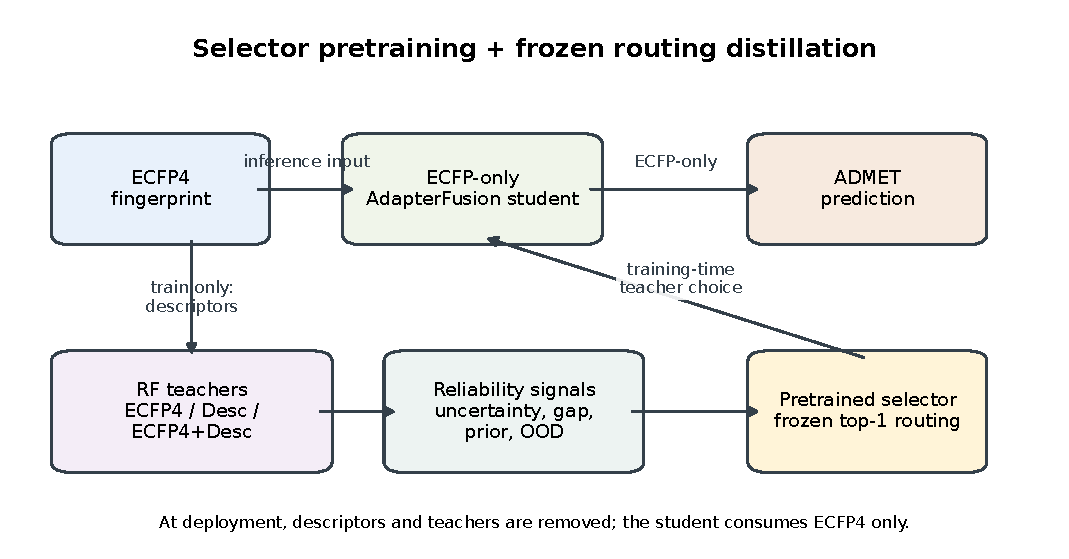
\includegraphics[width=\linewidth]{../paper_figures_second/fig1_selector_method.pdf}
\caption{Overview of pretrained teacher selection with frozen routing
distillation. During training, RF teachers and reliability signals supervise a
standalone selector; the frozen selector routes teacher supervision into an
ECFP-only AdapterFusion student. At inference, only ECFP4 is used.}
\label{fig:method}
\end{figure}

\subsection{ECFP-only AdapterFusion student}

The student follows an AdapterFusion backbone. An ECFP4 fingerprint is encoded
into \(z_{fp}\). A pseudo-descriptor adapter maps this representation into
\(z_{desc}\), and a learned gate fuses the two representations for target
prediction:
\[
z_{fp}=E(f(x)),\qquad z_{desc}=A(z_{fp}),
\]
\[
g=\sigma(G([z_{fp},z_{desc}])),\qquad
z_{fused}=g\odot z_{fp}+(1-g)\odot z_{desc}.
\]
The target head predicts from \(z_{fused}\), while the descriptor head predicts
\(d(x)\) during training. At inference, the model consumes only ECFP4.

\subsection{Molecular expert teachers}

The formal experiments use three random-forest teachers that expose different
molecular views: \texttt{ECFP4\_RF}, trained only on ECFP4 fingerprints;
\texttt{Desc\_RF}, trained only on standardized descriptors; and
\texttt{ECFP4\_Desc\_RF}, trained on concatenated ECFP4 and descriptor
features. These teachers provide a controlled setting in which the student
must choose among fingerprint-only, descriptor-only, and descriptor-access
supervision.

\subsection{Teacher-selection features}

For each molecule, the selector receives teacher-specific and shared
reliability features. For each teacher \(T_i\), these include RF uncertainty,
teacher consensus deviation
\[
\left|\hat{y}_i-\frac{1}{K}\sum_j\hat{y}_j\right|,
\]
and a validation-derived teacher prior computed from setting-level teacher validation RMSE. A shared
descriptor-space OOD distance is appended to the feature vector, following the
general QSAR concern that predictions are less reliable outside a model's
applicability domain \cite{Netzeva2005AD,Tropsha2010QSAR}. Teacher-student
disagreement is analyzed as a failure mode, but is not part of the formal
pretrained selector used in the main experiments.

\subsection{Cross-fit selector pretraining}

Within each dataset-ratio-seed training split, teachers are re-fit in
cross-validation folds to generate out-of-fold train predictions. The
pseudo-oracle selector label is the teacher with minimum absolute error on each
held-out train sample:
\[
y^{sel}(x)=\arg\min_i |\hat{y}_i(x)-y|.
\]
A random-forest classifier is trained on these labels with median imputation,
200 trees, maximum depth 8, and minimum leaf size 5. Logistic regression is
used only as a diagnostic baseline for selector predictability. The use of
out-of-fold labels follows the same leakage-control logic that underlies
standard QSAR validation practice \cite{Tropsha2010QSAR}.

\subsection{Frozen routing distillation}

After selector pretraining, the selector is frozen. For each training sample,
it outputs a probability distribution over teachers. The main method uses hard
top-1 routing:
\[
i^*(x)=\arg\max_i h_\phi(r(x))_i,\qquad
\mathcal{L}_{distill}=(\hat{y}_S-\hat{y}_{i^*(x)})^2.
\]
The selector is not updated during student training. This gives the student a
fixed teacher-selection signal rather than asking it to learn target
prediction and routing from the same low-resource loss.

\subsection{Training objective and ratio-aware calibration}

For regression, the student is trained with
\[
\mathcal{L}=\mathcal{L}_{task}
+\lambda_{desc}\mathcal{L}_{desc}
+\lambda_{mt}\sum_i w_i(x)(\hat{y}_S-\hat{y}_i)^2.
\]
For the main pretrained selector, \(w_i(x)\) is one-hot at the selected
teacher. For uniform and validation-weighted baselines, \(w_i(x)\) is either
uniform or derived from teacher validation RMSE. The default setting uses
\(\lambda_{desc}=0.1\) and \(\lambda_{mt}=1.0\).

The calibrated selector variant applies a train-ratio schedule:
\[
s(r)=
\begin{cases}
1.0, & r\in\{10,20\},\\
0.3, & r=50,
\end{cases}
\qquad
\lambda_{mt}^{eff}=\lambda_{mt}s(r).
\]
This high-resource decay tests whether selected teacher supervision should be
weakened once more labeled data are available.

\section{Experiments}

\subsection{Datasets and protocol}

The main experiments focus on regression ADMET prediction. We evaluate on five
endpoints: \texttt{caco2\_wang}, \texttt{lipophilicity\_astrazeneca},
\texttt{solubility\_aqsoldb}, \texttt{vdss\_lombardo}, and
\texttt{ppbr\_az}. These endpoints are drawn from the TDC and MoleculeNet
style molecular property benchmark ecosystem \cite{Wu2018MoleculeNet,Huang2021TDC};
for solubility, \texttt{solubility\_aqsoldb} traces to the AqSolDB resource
\cite{Sorkun2019AqSolDB}. We choose regression endpoints for the main study to
keep the selector target, distillation loss, and evaluation metric within a
single metric family. The selected endpoints cover absorption or permeability
(\texttt{caco2\_wang}), physicochemical properties (lipophilicity and
solubility), and distribution or binding (\texttt{vdss\_lombardo} and
\texttt{ppbr\_az}).
For each endpoint, we use 10\%, 20\%, and 50\% training
ratios with seeds 42, 123, and 3407, giving 45 dataset-ratio-seed settings.
The primary metric is test RMSE. Validation splits are used for teacher-prior
estimation, model selection, and setting-level teacher baselines, but the
pretrained selector's formal supervision comes from cross-fit pseudo-oracle
labels within the training split.

\subsection{Baselines}

We compare against several levels of teacher use. The first baseline is the
base ECFP-only AdapterFusion student with descriptor reconstruction but no
teacher distillation. The second is fixed single-teacher distillation from
\texttt{ECFP4\_Desc\_RF}. Multi-teacher controls include uniform averaging,
validation-weighted distillation, and \texttt{top1\_validation}, which selects
the best validation teacher for the entire dataset-ratio-seed setting. We also
keep the individual RF teachers, \texttt{ECFP4\_RF}, \texttt{Desc\_RF}, and
\texttt{ECFP4\_Desc\_RF}, as teacher controls.

\subsection{Main method}

The main method is pretrained selector hard top-1 routing. We additionally
report a calibrated variant with high-resource lambda decay, which keeps
distillation strength unchanged at 10\% and 20\% train ratios but reduces it
at 50\%. Selector-filtered and top-2 variants are treated as secondary
comparisons. Selector-confidence auto reweighting is reported only as a
diagnostic negative result.

\section{Results}

\subsection{Main regression results}

\begin{table}[t]
\centering
\small
\setlength{\tabcolsep}{3pt}
\begin{tabular}{lrrrrrrrrr}
\toprule
Method & RMSE & \(\Delta\) Base & Wins & \(\Delta\) Fixed & Wins & \(\Delta\) Top1 & Wins & \(\Delta\) Sel. & Wins \\
\midrule
Base AdapterFusion & 5.1841 & -- & -- & 0.0221 & 15/45 & 0.1049 & 11/45 & 0.0953 & 11/45 \\
Fixed ECFP4+Desc RF & 5.1621 & -0.0221 & 30/45 & -- & -- & 0.0828 & 19/45 & 0.0732 & 17/45 \\
Uniform multi-teacher & 5.1403 & -0.0438 & 29/45 & -0.0217 & 23/45 & 0.0611 & 24/45 & 0.0514 & 21/45 \\
Validation-weighted & 5.0969 & -0.0872 & 33/45 & -0.0651 & 24/45 & 0.0177 & 19/45 & 0.0081 & 19/45 \\
Top-1 validation & 5.0792 & -0.1049 & 34/45 & -0.0828 & 26/45 & -- & -- & -0.0096 & 20/45 \\
Pretrained selector & 5.0889 & -0.0953 & 34/45 & -0.0732 & 28/45 & 0.0096 & 25/45 & -- & -- \\
Selector + high-resource decay & 5.0814 & -0.1028 & 34/45 & -0.0807 & 32/45 & 0.0021 & 27/45 & -0.0075 & 9/45 \\
\bottomrule
\end{tabular}
\caption{Full 45-run regression comparison. RMSE is lower better. Deltas are
method minus reference, so negative values indicate improvement.}
\label{tab:main}
\end{table}

\begin{figure}[t]
\centering
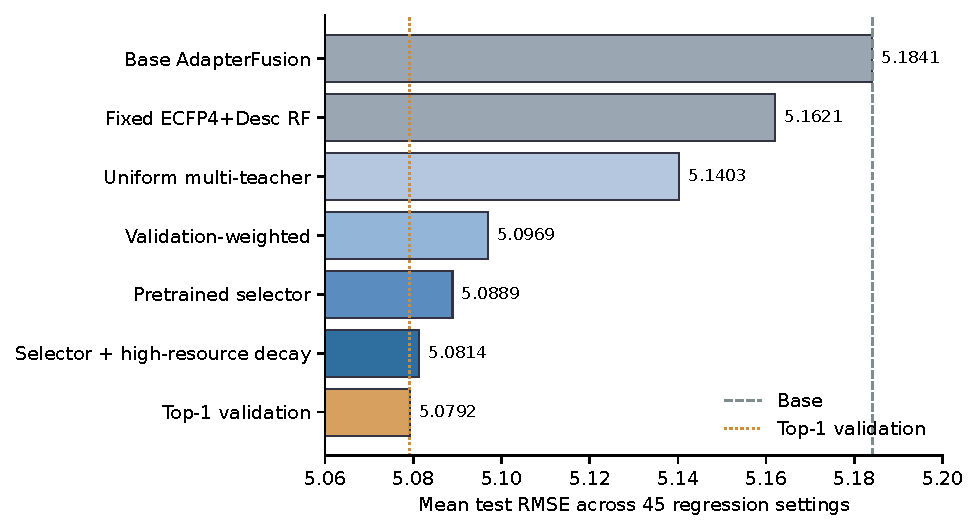
\includegraphics[width=0.88\linewidth]{../paper_figures_second/fig2_main_rmse.pdf}
\caption{Aggregate mean test RMSE across 45 regression settings. The
pretrained selector improves over base AdapterFusion and fixed single-teacher
distillation, while high-resource decay nearly matches the strong
\texttt{top1\_validation} baseline.}
\label{fig:main_rmse}
\end{figure}

Table~\ref{tab:main} summarizes the full regression matrix. The base ECFP-only
AdapterFusion student obtains a mean test RMSE of 5.1841. Fixed single-teacher
distillation from the descriptor-access \texttt{ECFP4\_Desc\_RF} teacher
improves this to 5.1621, confirming that descriptor-informed teacher
supervision can benefit an ECFP-only student. Uniform multi-teacher
distillation improves mean test RMSE to 5.1403, while validation-weighted
multi-teacher distillation improves it further to 5.0969. The best
setting-level baseline is \texttt{top1\_validation}, which reaches 5.0792 mean
test RMSE.

The proposed pretrained selector with frozen top-1 routing reaches 5.0889 mean
test RMSE. It improves over base AdapterFusion in 34 of 45 runs and over fixed
single-teacher distillation in 28 of 45 runs. Compared with
\texttt{top1\_validation}, the selector wins 25 of 45 runs but remains slightly
worse on average by +0.0096 RMSE. Thus, the selector closes most of the gap to
the strongest setting-level teacher selector, but it does not decisively
dominate that baseline.

Adding high-resource lambda decay further improves the pretrained selector. It
reaches 5.0814 mean test RMSE, improves over fixed distillation in 32 of 45
runs, and improves over the plain pretrained selector on mean RMSE by -0.0075.
It also wins against \texttt{top1\_validation} in 27 of 45 runs, although its
aggregate mean remains marginally higher than \texttt{top1\_validation} by
+0.0021 RMSE. We therefore treat high-resource decay as a useful calibration
of selector routing rather than as a separate main contribution.

\subsection{Dataset and train-ratio behavior}

The dataset-ratio results show that the benefit of selector routing is not
uniform. On \texttt{caco2\_wang}, the pretrained selector is strongest at 10\%
and 20\% train ratios, while high-resource decay improves the 50\% setting
relative to the plain selector. The same pattern appears on \texttt{ppbr\_az},
where the calibrated selector improves the 50\% setting from 14.4500 to
14.3472 mean RMSE and beats \texttt{top1\_validation} at that ratio.

For \texttt{lipophilicity\_astrazeneca}, pretrained selector routing is
strongest at 20\%, while the 50\% setting is still best served by fixed
descriptor-access teacher distillation. For \texttt{solubility\_\allowbreak aqsoldb}, the
differences among uniform multi-teacher, top-1 validation, and selector
routing are small. For \texttt{vdss\_lombardo}, base AdapterFusion remains
competitive in the 20\% and 50\% settings, and high-resource decay slightly
weakens the plain selector at 50\%. These endpoint differences show that
teacher selection is not reducible to a single globally best teacher or a
single globally best weighting rule.

\begin{figure}[t]
\centering
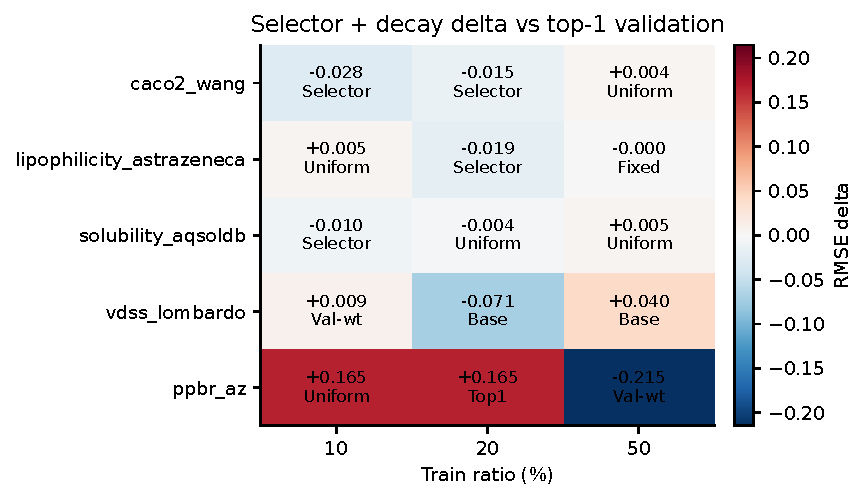
\includegraphics[width=0.82\linewidth]{../paper_figures_second/fig3_setting_delta_heatmap.pdf}
\caption{Dataset-ratio behavior of the calibrated selector. Each cell reports
the RMSE delta of selector plus high-resource decay relative to
\texttt{top1\_validation}; negative values favor the selector. Text inside
each cell shows the best method for that dataset-ratio setting.}
\label{fig:setting_delta}
\end{figure}

\subsection{Negative and secondary ablations}

\begin{table}[t]
\centering
\small
\begin{tabular}{llrrr}
\toprule
Method & Scope & RMSE & Wins & \(\Delta\) Plain \\
\midrule
Plain selector & 18 runs & 8.6091 & -- & -- \\
Auto confidence reweight & 18 runs & 8.7875 & 7/18 & 0.1783 \\
Low-resource decay & 18 runs & 8.6666 & 7/18 & 0.0575 \\
High-resource decay & 18 runs & 8.5852 & 5/18 & -0.0239 \\
\bottomrule
\end{tabular}
\caption{Secondary ablations on the \texttt{caco2\_wang} and \texttt{ppbr\_az}
partial regression subset. Wins are counted against the plain pretrained
selector. Negative deltas indicate lower mean RMSE than the plain selector.}
\label{tab:secondary_ablation}
\end{table}

Several alternatives were tested before settling on pretrained selector
routing. Table~\ref{tab:secondary_ablation} summarizes the main secondary
ablations. Joint learned gates and supervised joint gates were weak in smoke
experiments, indicating that simply adding a routing network to the student
does not provide a stable teacher-selection signal. Selector-confidence
auto-reweighting was reproducible and locally useful, but on the 18-run
\texttt{caco2\_wang} + \texttt{ppbr\_az} partial regression subset it
increased mean RMSE from 8.6091 to 8.7875 relative to the plain selector.

The ratio-aware lambda analysis gives a more useful secondary result. Early
lambda decay, which reduces distillation strength already at the 20\% train
ratio, is harmful on the same partial subset. High-resource decay is more
defensible because it leaves 10\% and 20\% settings unchanged and only weakens
teacher forcing at 50\%. On the full matrix, this improves the plain selector
from 5.0889 to 5.0814 mean RMSE.

\section{Mechanism Analysis}

\subsection{Teacher selection is predictable}

\begin{table}[t]
\centering
\small
\begin{tabular}{llr}
\toprule
Diagnostic & Scope & Value \\
\midrule
RF selector validation accuracy & 45 settings & 0.5178 \\
RF selector test accuracy & 45 settings & 0.5425 \\
RF selector validation macro-F1 & 45 settings & 0.4269 \\
RF selector test macro-F1 & 45 settings & 0.4396 \\
RF gate probe weighted accuracy & 45 leave-one-setting-out groups & 0.5617 \\
Logistic gate probe weighted accuracy & 45 leave-one-setting-out groups & 0.5044 \\
Majority-train weighted accuracy & 45 leave-one-setting-out groups & 0.4818 \\
Setting-prior top-1 weighted accuracy & 45 leave-one-setting-out groups & 0.4360 \\
\bottomrule
\end{tabular}
\caption{Selector predictability diagnostics.}
\label{tab:selector_diagnostics}
\end{table}

\begin{figure}[t]
\centering
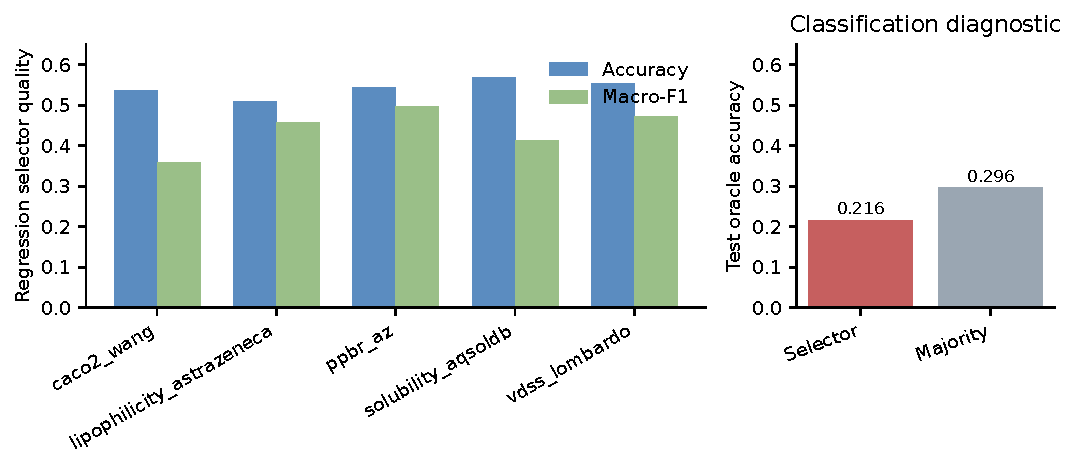
\includegraphics[width=\linewidth]{../paper_figures_second/fig4_selector_quality.pdf}
\caption{Selector quality diagnostics. Left: regression selector accuracy and
macro-F1 by endpoint. Right: the same selector protocol fails on classification
diagnostics, where test oracle-teacher accuracy is below the train-majority
baseline.}
\label{fig:selector_quality}
\end{figure}

The first mechanism question is whether teacher selection contains learnable
signal at all. Table~\ref{tab:selector_diagnostics} shows that a
random-forest gate probe reaches a weighted oracle-teacher accuracy of 0.5617
across 45 held-out settings. This substantially exceeds both the global
majority baseline (0.4818) and the setting-level prior baseline (0.4360). A
logistic probe also beats these baselines with 0.5044 weighted accuracy, but
is clearly weaker than the random-forest probe. The failure of joint gates is
therefore not caused by teacher reliability being random or unobservable;
rather, the issue is how the teacher-selection signal is supervised and
coupled to student optimization.

\subsection{Selector quality and failure modes}

The pretrained random-forest selector remains noisy, but its quality is stable
across the full regression matrix. Averaged over 45 settings, it obtains 0.5178
validation accuracy and 0.5425 test accuracy, with validation and test
macro-F1 of 0.4269 and 0.4396. These numbers are not high enough to treat the
selector as an oracle, but they are sufficient to route useful supervision into
the student.

The remaining gap to \texttt{top1\_validation} is small but informative. Some
settings are still better handled by a coarse setting-level teacher choice.
For example, \texttt{ppbr\_az} at 20\% train ratio strongly favors
\texttt{top1\_validation}, while the selector remains weaker despite strong
average selector accuracy on that endpoint. This suggests that selector
correctness against sample-level pseudo-oracle labels is not always aligned
with the student-level RMSE gained from routed distillation.

The high-resource lambda results show that teacher strength matters even after
teacher choice is fixed. At 50\% train ratio, reducing distillation strength
improves the calibrated selector mean RMSE from 4.6001 to 4.5774 across
datasets. At 10\% and 20\%, the calibrated method intentionally matches the
plain selector, because early weakening of teacher supervision hurt the
partial-regression results.

\subsection{Failure modes separate selection from utilization}

\begin{table}[H]
\centering
\small
\setlength{\tabcolsep}{3pt}
\begin{tabular}{llrrrrr}
\toprule
Setting & Subset & \(n\) & Sel. oracle & Top1 oracle & Sel. student wins & \(\Delta\) abs. err. \\
\midrule
\texttt{ppbr\_az} 20\% s42 & all & 559 & 0.5546 & 0.2576 & 0.3936 & +1.0748 \\
\texttt{ppbr\_az} 20\% s42 & sel.-better teacher & 251 & 0.9801 & 0.0000 & 0.3307 & +1.5003 \\
\texttt{caco2\_wang} 10\% s42 & all & 182 & 0.5714 & 0.5989 & 0.3736 & +0.0072 \\
\texttt{caco2\_wang} 10\% s42 & sel.-better teacher & 17 & 0.6471 & 0.0000 & 0.5294 & -0.0126 \\
\bottomrule
\end{tabular}
\caption{Failure-mode probes comparing teacher-selection correctness with
student-level benefit. ``Sel.-better teacher'' denotes disagreement samples
where the selector chooses a lower-error teacher than top-1 validation.
\(\Delta\) abs. err. is selector-routed student absolute error minus
top-1 validation student absolute error, so negative values favor the
selector-routed student.}
\label{tab:failure_probe}
\end{table}

Table~\ref{tab:failure_probe} separates two sources of the remaining gap. On
\texttt{ppbr\_az} at 20\% train ratio, the selector is substantially better
than top-1 validation at the teacher-selection problem itself
(0.5546 vs. 0.2576 oracle accuracy), and on disagreement samples where the
selector chooses the lower-error teacher it is nearly perfect. Yet the final
student is still worse, with a +1.5003 absolute-error delta on that subset.
This is a routing-utilization failure: better teacher choices are not reliably
converted into better student predictions.

The \texttt{caco2\_wang} probe shows the opposite pattern. There, the selector
does not beat top-1 validation on teacher-selection accuracy over the
full split, so the main bottleneck is selector quality. However, when the
selector does choose a better teacher on the disagreement subset, the student
effect is directionally positive. These probes support the central
interpretation that supervised teacher selection is useful, but future gains
require improving both selector quality and the way an ECFP-only student
absorbs routed teacher supervision.

\section{Discussion}

The main lesson from these experiments is that multi-teacher distillation for
low-resource ADMET should be treated as a teacher-selection problem, not only
as a teacher-averaging problem. Fixed descriptor-teacher distillation improves
the ECFP-only student, but it assumes that the same teacher and the same
distillation strength are appropriate across endpoints, train ratios, and
samples. The multi-teacher baselines show that this assumption is too coarse.
This is consistent with recent molecular learning work showing that multiple
views or auxiliary tasks can help, but that their value is not uniform across
settings \cite{Zheng2024MolFuse,Du2023MTGLADMET,Dey2024AuxAdapt}.

The proposed selector-pretraining strategy addresses a different failure mode
from standard adaptive weighting. Joint gates learn routing and target
prediction simultaneously, which makes them vulnerable to low-resource task
noise and early optimization dynamics. In contrast, the cross-fit selector is
trained with an explicit pseudo-oracle teacher-selection target before student
training begins. Freezing the selector then turns teacher choice into a stable
source of training-time supervision.

At the same time, selector accuracy alone is not the same as student
usefulness. A selector can correctly identify the teacher with the lowest
sample-level pseudo-oracle error, but the ECFP-only student may not benefit
equally from imitating that teacher. The method should therefore be read as
evidence that selector supervision is a useful missing ingredient, not as
evidence that sample-level routing has fully solved teacher reliability.

Descriptor-access RF teachers remain important controls. In several settings,
descriptor-access models or setting-level teacher choices still match or
exceed the ECFP-only student. The contribution of this work is not to claim
that ECFP-only inference universally dominates descriptor-access prediction.
Instead, it targets a deployment constraint: the student can use descriptors
and teacher predictions during training, but needs only ECFP4 at inference.
This complements graph and pretrained molecular representation learning
\cite{Yang2019DMPNN,Rong2020GROVER,Hu2020PretrainGNN,Liu2022GraphMVP,Heid2024Chemprop}
and recent cross-view molecular distillation work \cite{Zeng2024MolKD}
rather than replacing it; those models are natural candidates for future
teacher pools once the selector-supervision protocol is established.

\section{Limitations}

This study has several limitations. First, the main claim is restricted to
regression ADMET endpoints. Classification endpoints were explored in pilot
work but were less stable, and they should remain supplementary until the
teacher-selection protocol is evaluated under classification-specific metrics
and calibration behavior. In a five-endpoint classification diagnostic, the
same RF selector obtained only 0.2162 mean test oracle-teacher accuracy, below
the corresponding train-majority baseline of 0.2958, indicating that the
regression pseudo-oracle protocol should not be transferred directly to
classification tasks.

Second, the main dataset scope is deliberately restricted to regression
endpoints. This avoids mixing RMSE-based selector labels with
classification-specific calibration and ROC-AUC behavior, but it means the
current claim should be read as regression ADMET evidence rather than a complete
ADMET benchmark. Prepared classification endpoints such as blood-brain barrier
permeability, human intestinal absorption, P-gp interaction, bioavailability,
and hERG inhibition are natural supplementary diagnostics.

Third, the teacher set is deliberately limited. The main experiments use RF
teachers over ECFP4, descriptors, and their concatenation. This isolates the
teacher-selection problem, but it does not cover the full range of molecular
experts available in drug discovery. Adding XGBoost, graph neural networks, or
pretrained molecular encoders may change both the attainable student
performance and the difficulty of selecting among teachers.

Fourth, the selector features are partly hand-designed. Teacher uncertainty,
teacher consensus deviation, validation priors, and descriptor-space coverage
are interpretable and effective enough to predict pseudo-oracle teacher labels,
but they may not be optimal. Learned reliability representations or
meta-learned selector features could improve selection quality.

Fifth, the pseudo-oracle labels are based on teacher absolute error on
cross-fit predictions. This avoids direct leakage from fitting and evaluating
on the same samples, but it is still an imperfect proxy for the teacher that
will most improve the downstream student.

Finally, the calibrated high-resource lambda schedule is heuristic. It is
useful because it captures a clear pattern in the experiments, but it is not a
fully learned solution to teacher-strength calibration.

\section{Conclusion}

We presented pretrained teacher selection for reliable multi-teacher
distillation in low-resource ADMET. The method separates teacher-selection
supervision from student optimization by training a cross-fit pseudo-oracle
selector and freezing it for top-1 routing into an ECFP-only AdapterFusion
student. Across five regression endpoints, the selector improves over base and
fixed distillation and nearly matches a strong setting-level teacher selector.
The remaining gap highlights an important distinction: selecting a teacher,
choosing how strongly to imitate it, and obtaining student-level benefit are
related but distinct problems. This makes supervised teacher selection a
practical foundation for future ECFP-only molecular distillation systems.

\bibliographystyle{unsrt}
\bibliography{references}

\end{document}
